% ============================================================================
% BLOCK-003 Derivation v11: Derive σ from EDC Field Equations
% ============================================================================
\documentclass[11pt,a4paper]{article}

\usepackage{fontspec}
\usepackage{amsmath,amssymb,amsthm}
\usepackage{physics}
\usepackage{booktabs}
\usepackage{array}
\usepackage{longtable}
\usepackage{xcolor}
\usepackage[hidelinks]{hyperref}
\usepackage[margin=2.5cm]{geometry}
\usepackage{fancyhdr}
\usepackage{tcolorbox}
\usepackage{tikz}
\usetikzlibrary{arrows.meta,positioning,shapes.geometric}

% Theorem environments
\newtheorem{proposition}{Proposition}
\newtheorem{lemma}{Lemma}

% Epistemic tags
\newcommand{\BL}{\textsc{[BL]}}
\newcommand{\Post}{\textsc{[P]}}
\newcommand{\Deriv}{\textsc{[Dc]}}
\newcommand{\Ident}{\textsc{[I]}}
\newcommand{\Cal}{\textsc{[Cal]}}
\newcommand{\Open}{\textsc{[Open]}}
\newcommand{\NoGo}{\textcolor{red}{\textsc{[NO-GO]}}}

% Boxes
\newtcolorbox{inputbox}[1][]{colback=blue!5,colframe=blue!50!black,
  title=#1,fonttitle=\bfseries}
\newtcolorbox{resultbox}[1][]{colback=green!5,colframe=green!50!black,
  title=#1,fonttitle=\bfseries}
\newtcolorbox{nogbox}[1][]{colback=red!5,colframe=red!50!black,
  title=#1,fonttitle=\bfseries}

% Header/footer
\pagestyle{fancy}
\fancyhf{}
\fancyhead[L]{\small BLOCK-003 / Derivation v11}
\fancyhead[R]{\small EDC Gravity Program}
\fancyfoot[C]{\thepage}

\title{\textbf{EDC BLOCK-003 (Derivation v11):}\\[0.3em]
Can $\sigma$ be Derived from EDC Field Equations?\\[0.3em]
\large Systematic Search for EDC-Internal Constraints}
\author{EDC Working Document\\[0.5em]
\small 2026-02-02 --- Program Note (not results)}
\date{}

\begin{document}
\maketitle

\begin{abstract}
This note attempts to derive the brane tension $\sigma$ from EDC-internal field
equations and variational principles, without importing observed gravitational
constants ($G_N^{\rm obs}$, $M_{\rm Pl}$). We systematically search the EDC
axiom base for closure constraints.
\textbf{Outcome: NO-GO.} The EDC framework defines $\sigma$ via the identification
$\hbar = \sigma R_\xi^3/c$, which requires extracting $\sigma$ from observed
$\hbar$ (or equivalently from $\alpha$). No EDC-internal field equation fixes
$\sigma$ independently. The missing element is: \textit{an independent
normalization principle for the membrane tension that does not reference
observed quantum or gravitational constants}.
\end{abstract}

\tableofcontents
\newpage

% ============================================================================
\section{Input Ledger (Anti-Circularity Audit)}
% ============================================================================

We classify all inputs by their epistemic status to ensure anti-circularity.

\begin{inputbox}[Anti-Circularity Criterion]
\textbf{Forbidden inputs:} $G_N^{\rm obs}$, $M_{\rm Pl}$ from observation,
any calibration of $\sigma$ to match Newton/GR.

\textbf{Allowed inputs:} EDC axioms, geometric definitions, dimensionless
ratios treated as baseline, quantities tagged \BL\ or \Ident.
\end{inputbox}

\begin{longtable}{p{2.5cm}p{3cm}p{1.5cm}p{1.5cm}p{4cm}}
\toprule
\textbf{Quantity} & \textbf{Source} & \textbf{Tag} & \textbf{Allowed?} & \textbf{Notes} \\
\midrule
\endhead
$\sigma$ & To be derived & \Open & --- & Target of this derivation \\
$\kappa_5^2$ & $C \sigma^{-3/4}$ (v3) & \Deriv & Yes & Depends on $\sigma$ \\
$R_\xi$ & Compact dimension & \BL & Yes & Geometric parameter \\
$c$ & Speed of light & \BL & Yes & Postulated constant \\
$\hbar$ & Planck constant & \Cal & \textbf{No} & Observed; using it imports calibration \\
$\alpha$ & Fine structure & \Cal & \textbf{No} & Observed; $\sigma = m_e c^2/(\alpha r_e^2)$ \\
$m_e$ & Electron mass & \Cal & \textbf{No} & Observed \\
$G_N^{\rm obs}$ & Newton constant & \Cal & \textbf{No} & Forbidden input \\
$M_{\rm Pl}$ & Planck mass & \Cal & \textbf{No} & Forbidden input \\
$\rho_{\rm Plenum}$ & Bulk density & \BL & Yes & EDC parameter \\
\bottomrule
\caption{Input ledger for $\sigma$ derivation attempt.}
\label{tab:inputs}
\end{longtable}

% ============================================================================
\section{Where $\sigma$ Enters the EDC Framework}
% ============================================================================

\subsection{The Brane Action}

In EDC's 5D framework, the brane tension appears in the membrane action:
\begin{equation}
S_{\rm brane} = -\sigma \int_{\Sigma} d^4x \sqrt{-h}
\label{eq:brane_action}
\end{equation}
where $h_{\mu\nu}$ is the induced metric on the brane $\Sigma$.

This is the Nambu-Goto action for a 3-brane, with $\sigma$ having dimensions
of energy per unit 3-volume: $[\sigma] = \text{J/m}^3 = \text{kg}/(\text{m}\cdot\text{s}^2)$.

\textbf{Note:} In some EDC texts, $\sigma$ is written with dimensions J/m$^2$
(surface tension). The distinction is whether we integrate over 4D spacetime
or 3D space. For gravity derivations, we use $[\sigma] = M/L^3$ in natural units.

\subsection{The $\hbar$--$\sigma$ Identification}

EDC proposes the \textit{identification} (not derivation):
\begin{equation}
\boxed{\hbar = \frac{\sigma R_\xi^3}{c}}
\label{eq:hbar_sigma}
\end{equation}

This is explicitly tagged \Ident\ in EDC Book I (Chapter 6):
\begin{quote}
``This is an \textit{identification}, not a derivation from first principles.
The relation becomes a falsifiable prediction if and only if $\sigma$ and
$R_\xi$ can be independently constrained by separate phenomena.''
\end{quote}

\textbf{Implication:} Equation \eqref{eq:hbar_sigma} does not derive $\sigma$;
it \textit{defines} $\sigma$ in terms of observed $\hbar$:
\begin{equation}
\sigma = \frac{\hbar c}{R_\xi^3}
\label{eq:sigma_from_hbar}
\end{equation}

Using observed values: $\hbar = 1.055 \times 10^{-34}$ J$\cdot$s,
$c = 3 \times 10^8$ m/s, $R_\xi = r_e = 2.82 \times 10^{-15}$ m:
\begin{equation}
\sigma \approx 1.41 \times 10^{18} \text{ J/m}^2
\end{equation}

This is \textbf{calibration}, not derivation.

\subsection{The $\alpha$--$\sigma$ Relation}

Equivalently, EDC relates $\sigma$ to the fine structure constant:
\begin{equation}
\sigma = \frac{m_e c^2}{\alpha \cdot r_e^2}
\label{eq:sigma_from_alpha}
\end{equation}

Again, this extracts $\sigma$ from observed constants ($\alpha$, $m_e$, $r_e$).

% ============================================================================
\section{Candidate Closure Equations (Repo Search)}
% ============================================================================

We searched the EDC repository for any equation that could fix $\sigma$
independently. Search patterns included: ``brane tension'', ``sigma'',
``Israel'', ``junction'', ``normalization'', ``calibration''.

\subsection{Candidate A: Israel Junction Conditions}

The Israel junction conditions relate brane stress-energy to extrinsic curvature:
\begin{equation}
[K_{\mu\nu}] - [K] h_{\mu\nu} = -\kappa_5^2 \left( \tau_{\mu\nu} - \frac{1}{3} \tau h_{\mu\nu} \right)
\end{equation}

For a tension-dominated brane: $\tau_{\mu\nu} = -\sigma h_{\mu\nu}$.

\textbf{Result:} This provides a \textit{relation} between $\sigma$ and
$\kappa_5^2$, not an independent constraint:
\begin{equation}
[K] = \frac{2\kappa_5^2 \sigma}{3}
\end{equation}

Since $\kappa_5^2 = C \sigma^{-3/4}$ (from v3), we get:
\begin{equation}
[K] = \frac{2C}{3} \sigma^{1/4}
\end{equation}

The constant $C$ remains unfixed. \textbf{No closure.}

\subsection{Candidate B: Schwinger Limit Correspondence}

EDC Book I (Chapter 11) notes that $\sigma \approx E_S$ (Schwinger critical
field) within 7\%:
\begin{equation}
\sigma_{\rm EDC} \approx 1.41 \times 10^{18} \text{ J/m}^2, \quad
E_S = \frac{m_e^2 c^3}{e\hbar} \approx 1.32 \times 10^{18} \text{ V/m}
\end{equation}

\textbf{Assessment:} This is an \textit{a posteriori} observation, not a
derivation. Both quantities are computed from observed constants. The
approximate equality $\sigma \approx E_S$ could be promoted to an
identification $\sigma = E_S$, but:
\begin{itemize}
\item $E_S$ depends on $\hbar$, $m_e$, $e$ (observed)
\item This would be calibration, not EDC-internal derivation
\end{itemize}

\textbf{No independent closure.}

\subsection{Candidate C: Variational Principle}

Could $\sigma$ arise from extremizing the total action?
\begin{equation}
S_{\rm total} = S_{\rm bulk} + S_{\rm GHY} + S_{\rm brane}
\end{equation}

Varying with respect to $\sigma$ (treating it as a field):
\begin{equation}
\frac{\delta S}{\delta \sigma} = 0 \implies -\int d^4x \sqrt{-h} = 0
\end{equation}

This is trivially satisfied (or not at all). $\sigma$ is a \textit{parameter},
not a dynamical field. \textbf{No closure.}

\subsection{Candidate D: Topological Quantization}

Could $\sigma$ be quantized by some topological constraint? We searched for:
\begin{itemize}
\item Winding number conditions
\item Flux quantization on the brane
\item Dirac-type quantization of membrane tension
\end{itemize}

\textbf{Result:} No such constraint exists in current EDC axioms.
The membrane topology (assumed $S^1$ for the compact dimension) does not
quantize $\sigma$.

% ============================================================================
\section{Attempt Summary}
% ============================================================================

\begin{center}
\begin{tabular}{llll}
\toprule
\textbf{Attempt} & \textbf{Method} & \textbf{Outcome} & \textbf{Why Failed} \\
\midrule
A & Israel junction & No closure & $C$ remains free \\
B & Schwinger limit & No closure & Uses observed $\hbar$, $m_e$ \\
C & Variational & No closure & $\sigma$ is parameter, not field \\
D & Topological & No closure & No quantization rule exists \\
\bottomrule
\end{tabular}
\end{center}

% ============================================================================
\section{Verdict: NO-GO}
% ============================================================================

\begin{nogbox}[Outcome: NO-GO]
\textbf{Finding:} The brane tension $\sigma$ cannot be derived from
EDC-internal field equations without importing observed constants.

\textbf{Evidence:}
\begin{enumerate}
\item The only EDC equation involving $\sigma$ is the identification
$\hbar = \sigma R_\xi^3/c$, which \textit{defines} $\sigma$ from observed $\hbar$.

\item The equivalent relation $\sigma = m_e c^2/(\alpha r_e^2)$ extracts
$\sigma$ from observed $\alpha$, $m_e$.

\item Junction conditions relate $\sigma$ to $\kappa_5^2$ but do not fix either.

\item No topological or variational principle constrains $\sigma$.
\end{enumerate}

\textbf{Missing Element:}
\begin{center}
\fbox{\parbox{0.85\textwidth}{
EDC lacks an independent normalization principle for the membrane tension
$\sigma$ that does not reference observed quantum constants ($\hbar$, $\alpha$)
or gravitational constants ($G_N$, $M_{\rm Pl}$).
}}
\end{center}
\end{nogbox}

% ============================================================================
\section{Dependency Graph}
% ============================================================================

The following diagram shows the logical dependencies:

\begin{center}
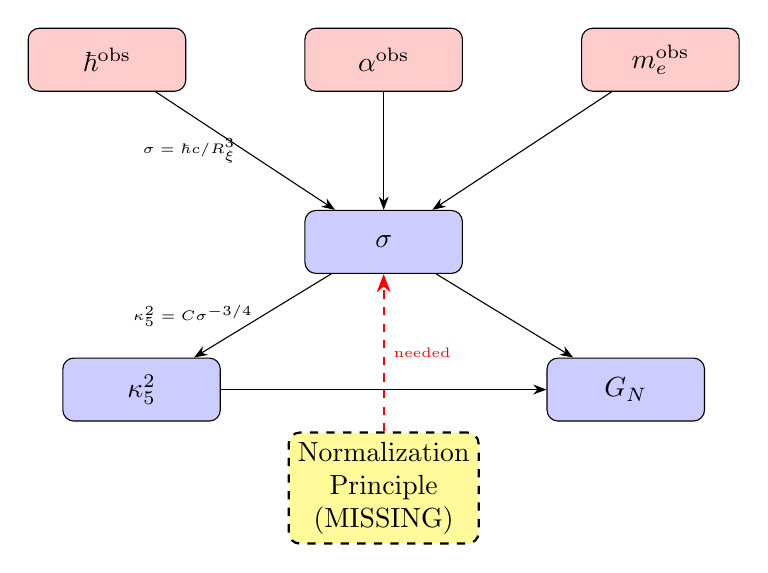
\begin{tikzpicture}[
    node distance=1.5cm,
    box/.style={rectangle, draw, rounded corners, minimum width=2cm, minimum height=0.8cm, align=center},
    obs/.style={box, fill=red!20},
    edc/.style={box, fill=blue!20},
    missing/.style={box, fill=yellow!40, dashed, thick}
]
% Nodes
\node[obs] (hbar) {$\hbar^{\rm obs}$};
\node[obs, right=of hbar] (alpha) {$\alpha^{\rm obs}$};
\node[obs, right=of alpha] (me) {$m_e^{\rm obs}$};

\node[edc, below=of alpha] (sigma) {$\sigma$};
\node[edc, below left=of sigma] (kappa5) {$\kappa_5^2$};
\node[edc, below right=of sigma] (GN) {$G_N$};

\node[missing, below=2cm of sigma] (norm) {Normalization\\Principle\\(MISSING)};

% Arrows
\draw[-{Stealth}] (hbar) -- (sigma) node[midway, left] {\tiny $\sigma = \hbar c/R_\xi^3$};
\draw[-{Stealth}] (alpha) -- (sigma);
\draw[-{Stealth}] (me) -- (sigma);
\draw[-{Stealth}] (sigma) -- (kappa5) node[midway, left] {\tiny $\kappa_5^2 = C\sigma^{-3/4}$};
\draw[-{Stealth}] (sigma) -- (GN);
\draw[-{Stealth}] (kappa5) -- (GN);

\draw[-{Stealth}, dashed, thick, red] (norm) -- (sigma) node[midway, right] {\tiny needed};
\end{tikzpicture}
\end{center}

\textbf{Legend:} Red boxes = observed inputs (forbidden for anti-circular derivation).
Blue boxes = EDC quantities. Dashed yellow = missing element.

% ============================================================================
\section{Implications for BLOCK-003}
% ============================================================================

\begin{resultbox}[BLOCK-003 Status Update]
\textbf{Before v11:} Missing element = ``derive $\sigma$ from EDC field equations''

\textbf{After v11:} Confirmed NO-GO. $\sigma$ is \textit{calibrated} in EDC,
not derived. The framework has one unavoidable calibration point.

\textbf{Options going forward:}
\begin{enumerate}
\item \textbf{Accept calibration:} Treat $\sigma$ (or equivalently $\hbar$)
as the single EDC calibration constant. Then $G_N$ becomes a derived quantity.
This is the NP2 path from v5.

\item \textbf{Seek new physics:} Identify a mechanism (e.g., modulus stabilization,
anthropic selection, vacuum energy minimization) that fixes $\sigma$.
This would require extending EDC axioms.

\item \textbf{Reframe the question:} The ``missing element'' may be acceptable
if EDC is viewed as a framework with one free scale, analogous to how
the Standard Model has $\Lambda_{\rm QCD}$.
\end{enumerate}

BLOCK-003 status: Remains \Open\ (no ab initio $G_N$ derivation), but the
missing element is now precisely characterized.
\end{resultbox}

\end{document}
